\documentclass{article}

\usepackage{graphicx}
\usepackage{wrapfig}
\usepackage{float}
\usepackage{parskip}
\graphicspath{ {./images/} }

% Language setting
% Replace `english' with e.g. `spanish' to change the document language
\usepackage[english]{babel}

% Allow for sub sub section use

% Set page size and margins
% Replace `letterpaper' with `a4paper' for UK/EU standard size
\usepackage[letterpaper,top=2cm,bottom=2cm,left=3cm,right=3cm,marginparwidth=1.75cm]{geometry}

% Useful packages
\usepackage{amsmath}
\usepackage{graphicx}
\usepackage[colorlinks=true, allcolors=blue]{hyperref}
\usepackage{caption}
\usepackage{subcaption}


\title{ARMv8 AArch64\\
       \large Final Report - Group 25}
\author{
        Bogdan Gavra \\
        Michał Andryskowski\\
        Jakub Łapiński\\
        Vlad Marchis\\\\
        Mentor: 
        Matthew Baugh
        }

\begin{document}
\maketitle
\section{Assembler}
Similarly to the emulator, the assembler was structured in four general parts: the overarching \textbf{assembler}, the \textbf{controller}, the \textbf{instruction types}, and the \textbf{utility} files. The chosen label handling method is the \textit{Two-pass} algorithm, generating the symbol table in the first pass, and then replacing them with memory addresses in the second.\par
The program was organized such that, upon running the executable, the following steps would be run:
\begin{enumerate}
    \item The input file is split into lines, with empty lines and comments (lines beginning with the '\#' character) being ignored, while the labels are replaced with immediate values generated in the aforementioned label processing auxiliary function.
    \item The program then iterates through the lines in the same order as their appearance in the input file, and for each line, it calls the main controller function.
    \item The controller replaces the aliases (if they exist) with their expanded version, gets the instruction type (DPI, SDT, Branch, Special), and calls the corresponding function from the \textbf{/instruction} directory.
    \item The 32-bit instruction mask is then passed back to the main assembler function, which stores it in the given output file.
\end{enumerate}
In order to have easy debugging in the off-chance of a memory leak, we kept the memory allocation to a minimum throughout this project. Furthermore, we tried to minimize the amount of content and add comments, so that the code is readable.

\section{Extension - "The DOC Archives: \textit{Konstantinos' Destiny}"}

\subsection{Introduction}
Given the time remaining after implementing the first two parts of the project, we decided on developing a more challenging extension: a game. We wanted something enjoyable which would also leverage the team's previous expertise: rendering, game physics, and algorithms. We also wished to make something appealing to first-year Computing students, integrating all sorts of references, whilst having a practical use: gamifying studying for exams.
\subsection{Game description}
We settled on a rogue-like dungeon crawler, having Konstantinos, the first-year principal teaching fellow, as the playable main character. He moves through multiple rooms (resembling the Huxley building labs), facing all sorts of technological threats and answering different questions in order to gain power-ups, until facing the final boss, a personification of Haskell corrupted by ChatGPT. Moreover, due to the educational aspect of this game, the difficulty exponentially increases if he chooses not to answer the questions encountered, which would incentivize the player not to skip them.

\begin{figure}[H]
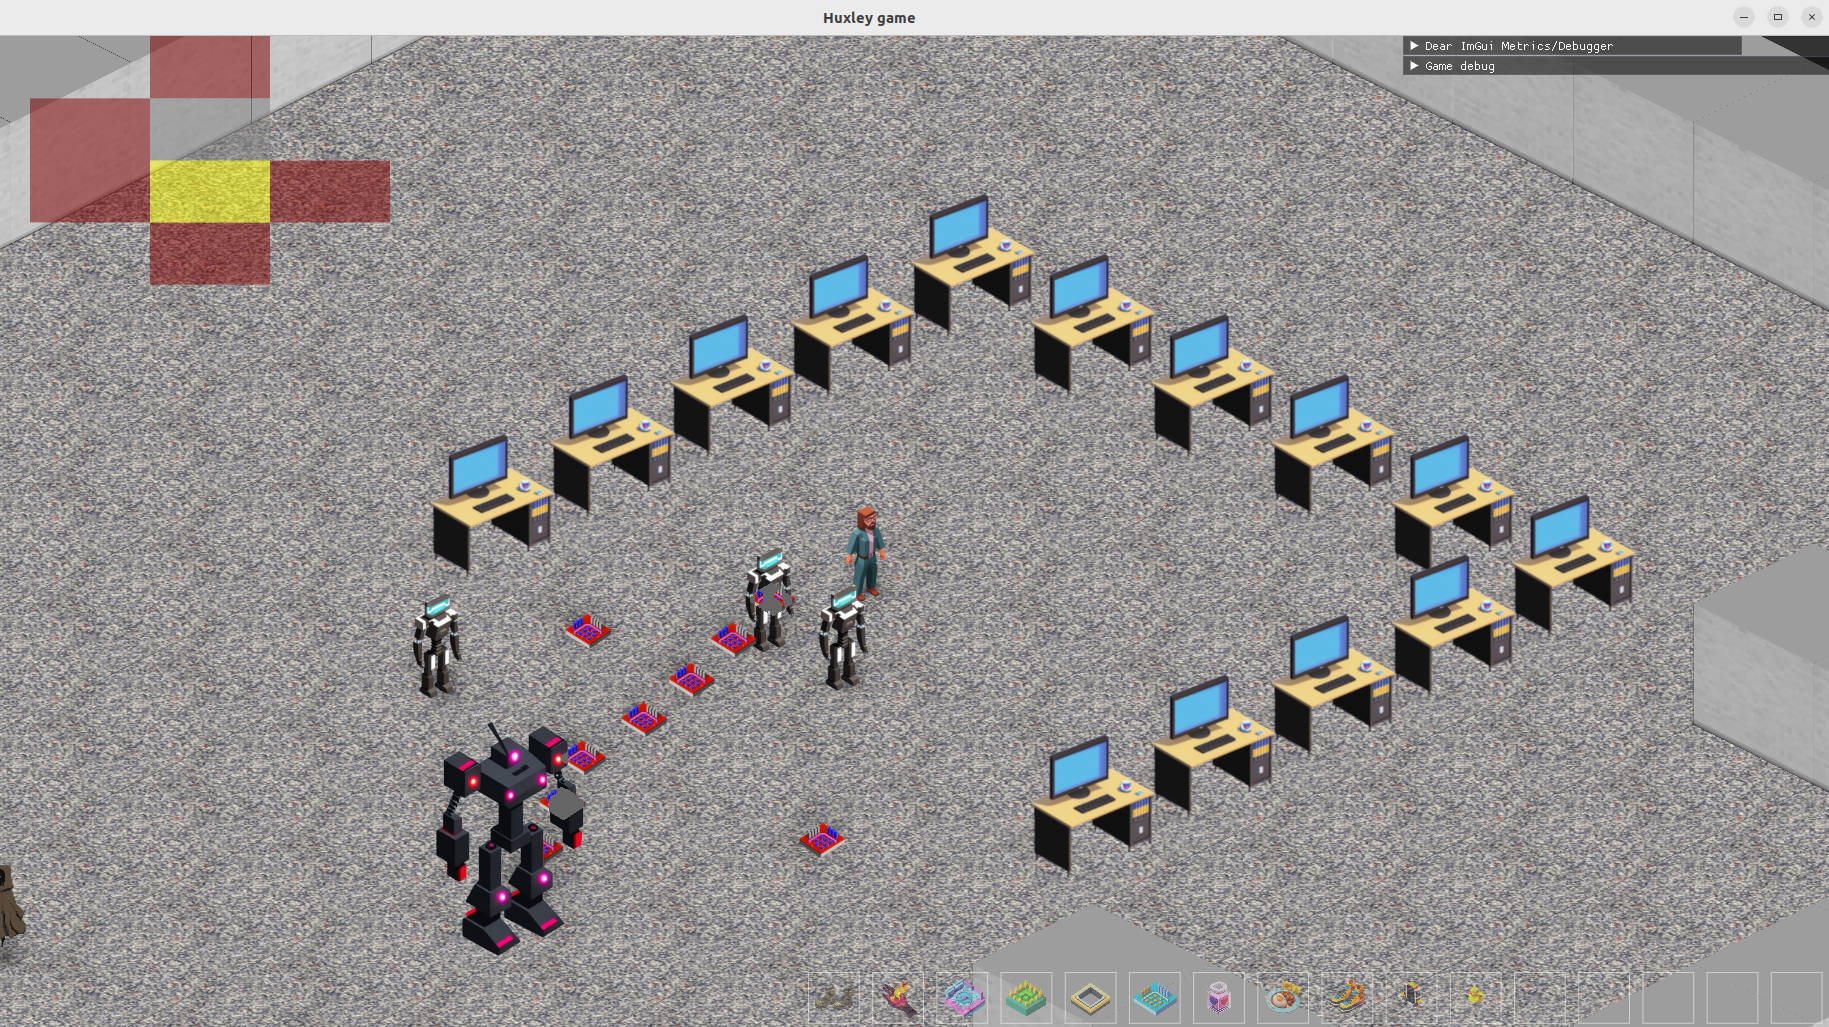
\includegraphics[scale=0.2]{images/gamePreview.png}
\centering
\caption{\textit{A preview of the gameplay (main character centered).}}
\end{figure}


\subsection{Game implementation}

\subsubsection{Rendering}
Given the narrow time frame, the scope of the game had to be limited in all areas, including rendering and art. To simplify rendering and room generation the in-game rooms are rendered as 2D grids of textured quads. It was essential to set up at least a basic tile renderer quickly so that the rest of the group could debug their features and receive visual feedback. \par
The renderer pre-generates a 2D grid of quads corresponding to each tile in the room with already pre-set texture IDs and sends it to the GPU. \par
Once we got it working we quickly realized that the same idea can be applied to set up an isometric renderer. This was a major stepping stone in the development of the game, which made it look more polished at a low cost. We found plenty of public-domain isometric assets which was also a plus. \par
To save time, we use one shader with multiple material types. We used the \textbf{depth buffer}, normally found in 3D rendering so that we can give an illusion of depth with 2D assets. Each tile is given a depth based on its x and y position so that entities can be obstructed by walls and vice versa.


\begin{figure}[H]
\centering
\begin{subfigure}{.30\textwidth}
  \centering
  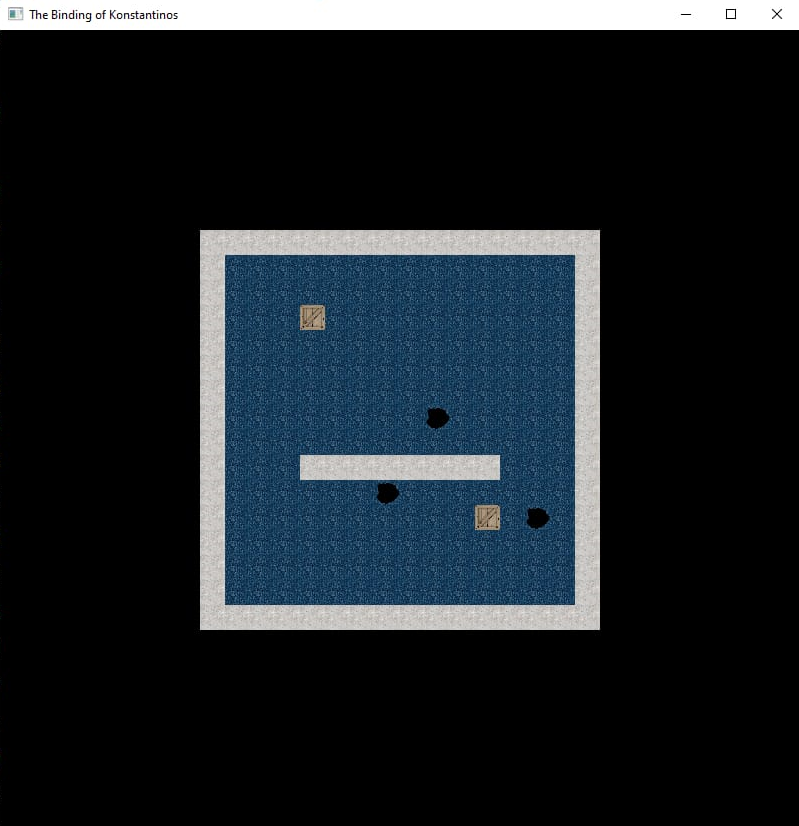
\includegraphics[width=0.9\linewidth]{images/firstRender.png}
  \caption{First tile renderer}
  \label{fig:sub1}
\end{subfigure}%
\begin{subfigure}{.30\textwidth}
  \centering
  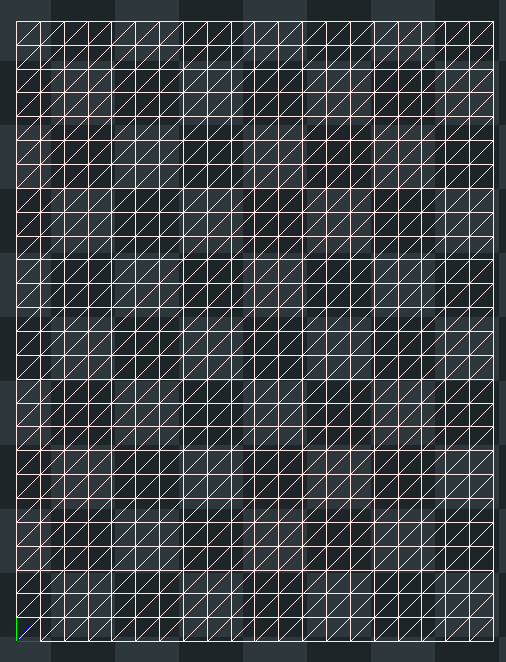
\includegraphics[width=0.65\linewidth]{images/gridRender.png}
  \caption{Grid of quads}
  \label{fig:sub2}
\end{subfigure}%
\begin{subfigure}{.30\textwidth}
  \centering
  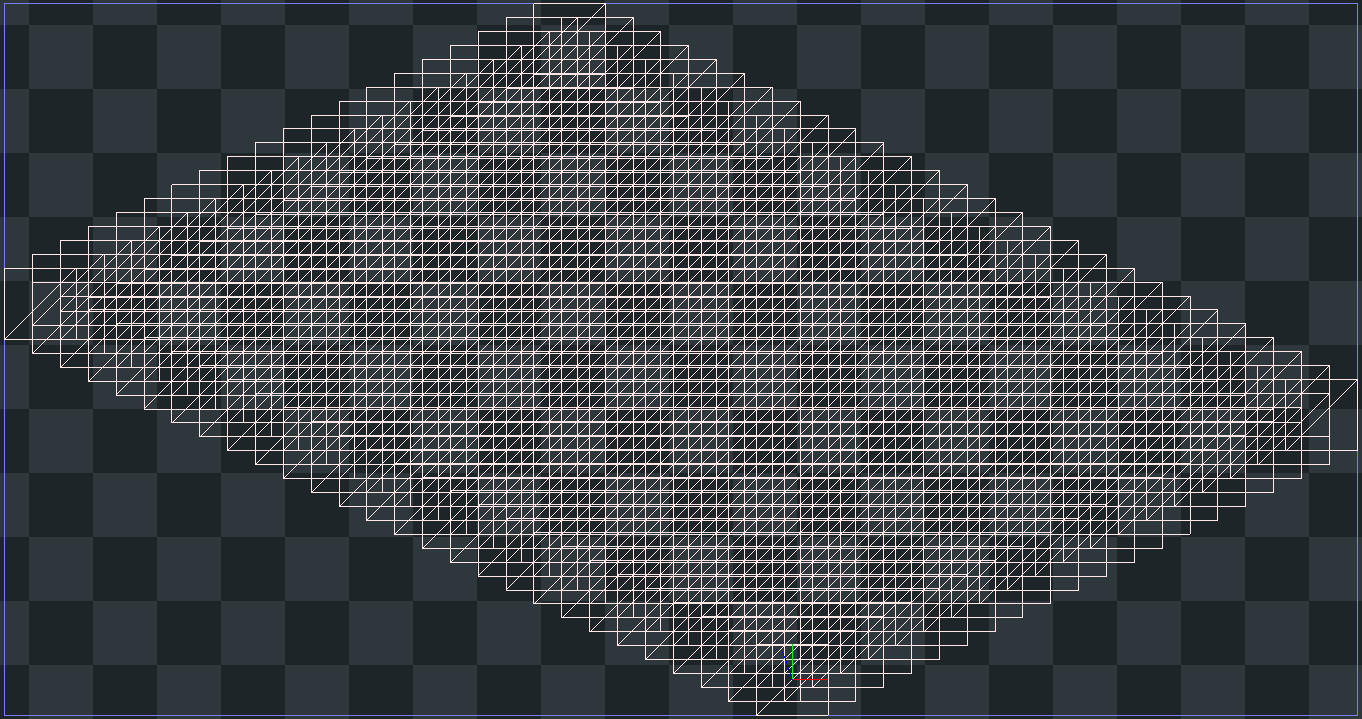
\includegraphics[width=1.0\linewidth]{images/isoRender.png}
  \caption{Grid of quads for isometric}
  \label{fig:sub3}
\end{subfigure}
\caption{Tile rendering}
\label{fig:test}
\end{figure}

\subsubsection{Room generation}
The parameters defining a room are \textbf{type} and \textbf{gamemode}(difficulty). Based on its type, a room can be randomly generated (using a set of predefined structures that are arbitrarily resized and placed) or preset (e.g. Boss, Item, Shop, etc.). The preset rooms were inspired by the game we used as a reference (Fig. 3). The doors are added last after the map structure is generated.\par
When it comes to spawning monsters, the difficulty determines their type and amount. Using a two-pass algorithm we calculate a spawn chance grid in terms of their positioning (in relation to the entry points of the room) and then place them throughout the map, with a higher chance of them spawning closer to the center of the room.
\begin{figure}[H]
\centering
\begin{subfigure}{.5\textwidth}
  \centering
  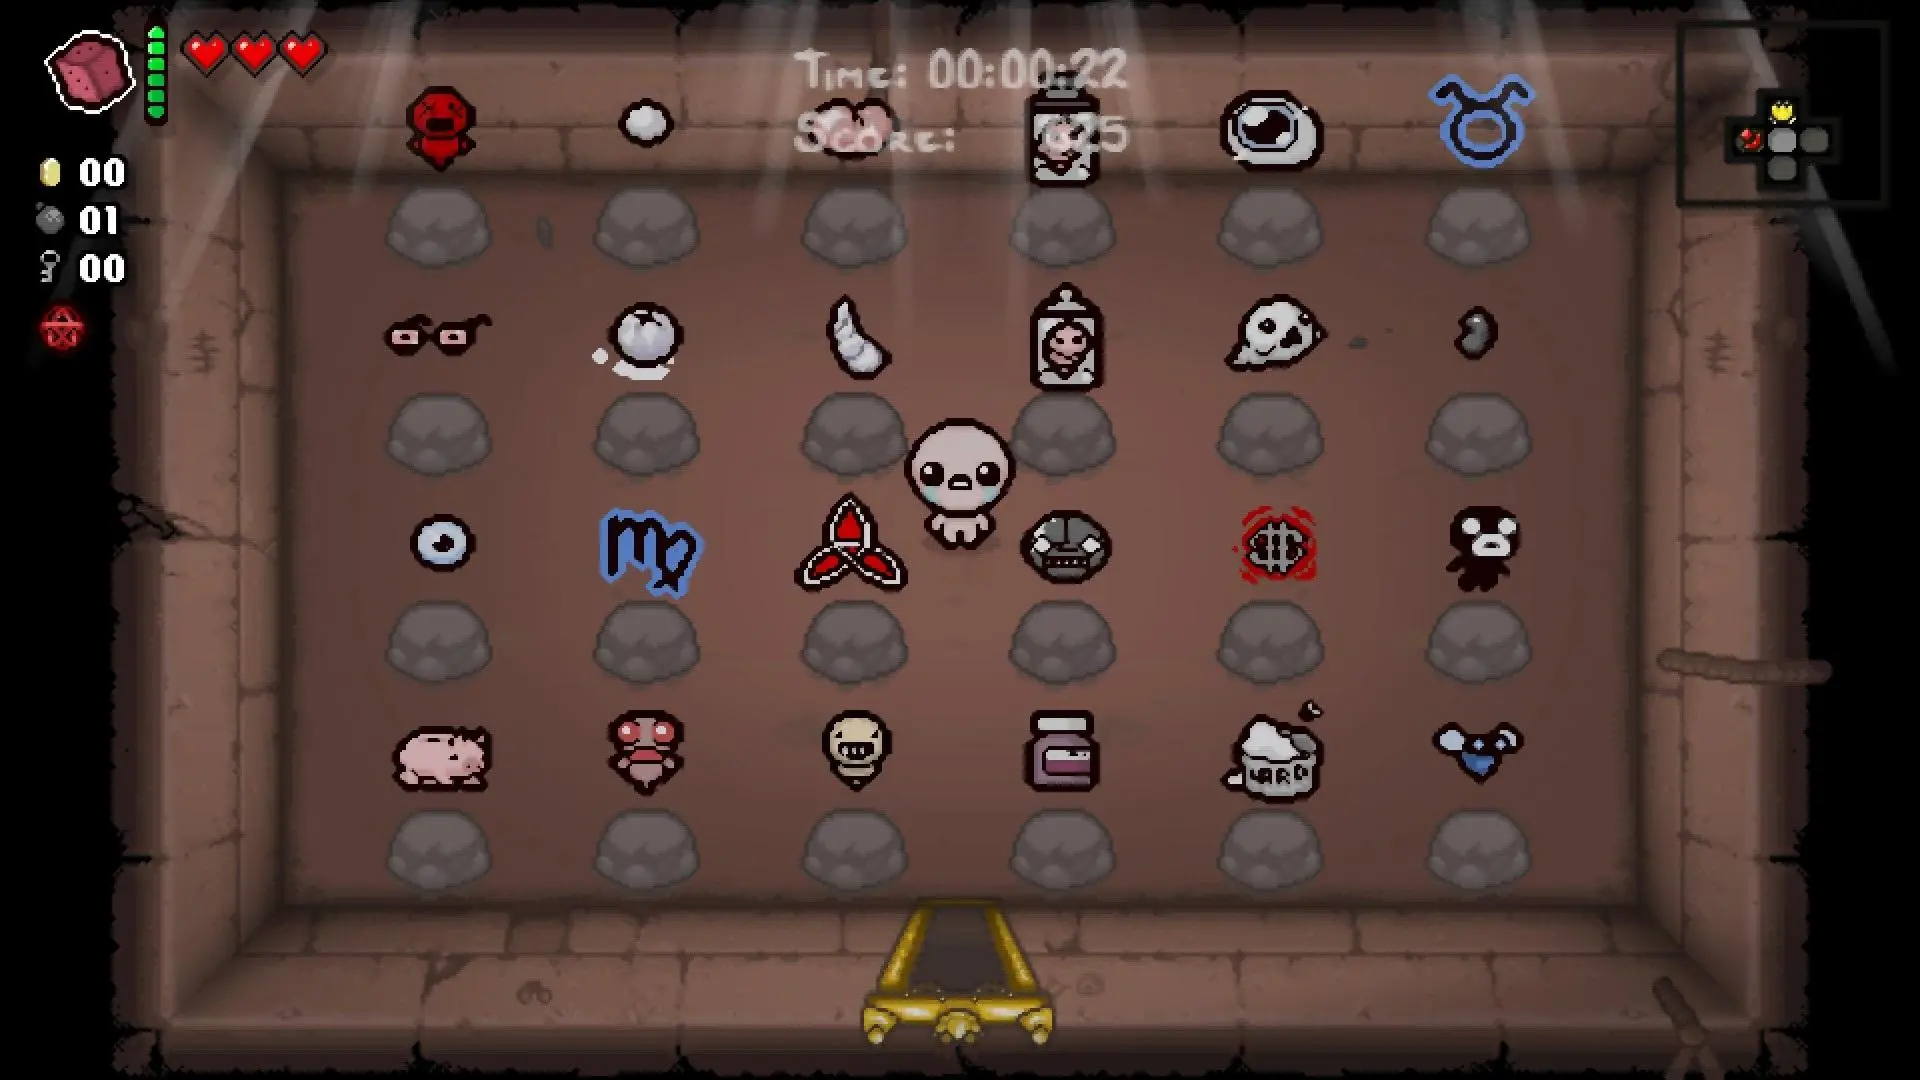
\includegraphics[width=0.9\linewidth]{images/checkeredRoom.png}
  \caption{Checkered item room}
  \label{fig:sub4}
\end{subfigure}%
\begin{subfigure}{.5\textwidth}
  \centering
  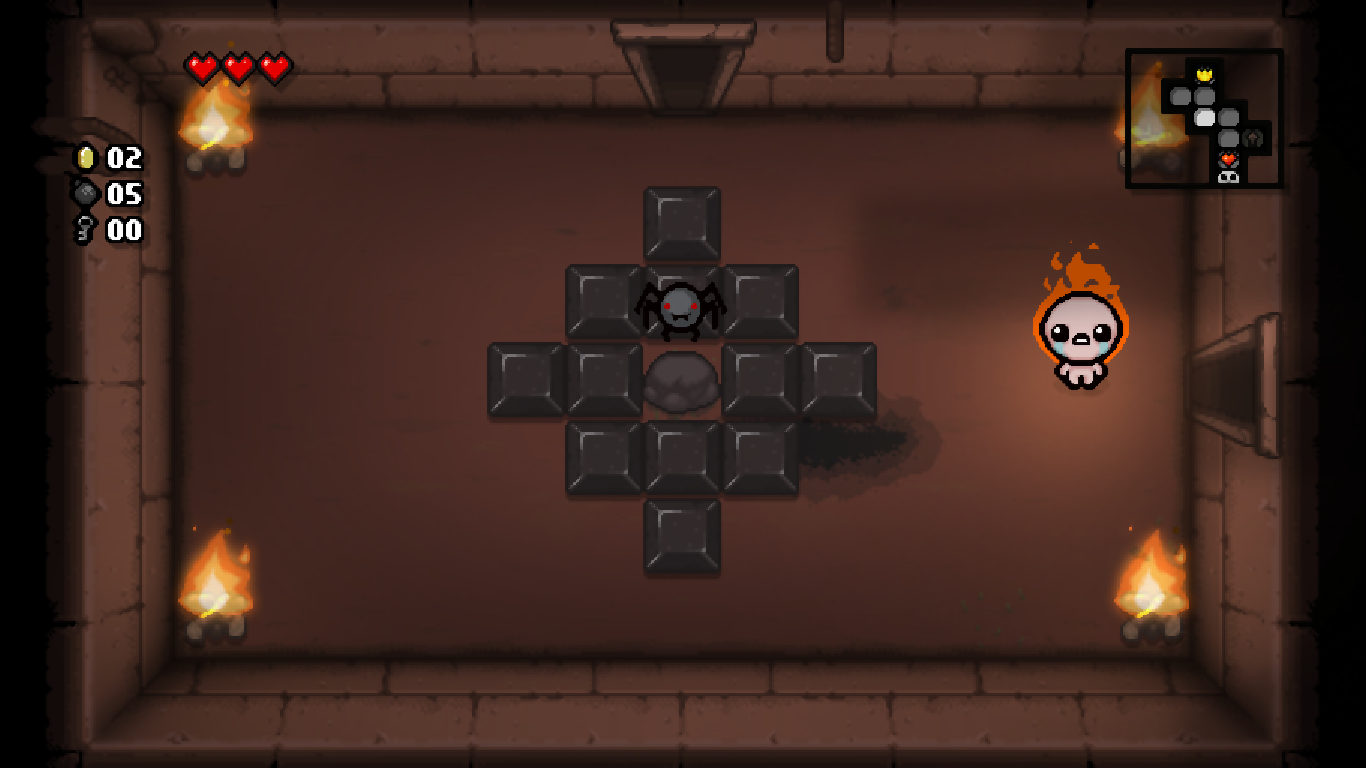
\includegraphics[width=0.9\linewidth]{images/randomTile.png}
  \caption{Random tiled room}
  \label{fig:sub5}
\end{subfigure}
\caption{Rooms from the game \textit{Binding of Isaac (2011)}}
\label{fig:test2}
\end{figure}

\subsubsection{Items + Special rooms}
In order for there to be a natural progression, the player had to obtain power-ups. Thus, items were introduced to the game, which either increased the players' base attributes or gave them special abilities (bouncing projectiles, bomb trail, turning back time). For balance, we decided to make these items obtainable only in special rooms: \textbf{The Shop} and \textbf{The Treasury}. The treasury contains a free randomized item that the player can choose to collect, while the shop provides the player with the chance to spend the coins collected throughout the run, giving him 3 different options, as well as the opportunity to refresh the item pool, all with a certain cost.
\subsubsection{Entities}
Due to the lack of \textbf{Object-Oriented Programming} (OOP) features in C, we had to improvise when implementing the entities,
leveraging function pointers for their actions, as well as trying to generalize everything inherited by the entity. The player is a structure that has \textit{unique fields} (such as movement swing, coin count, item lists), but which also contains an \textit{Entity} field, in order to make the movement much easier to implement. Overall, some shortcuts were taken in order to make the project in the short time frame available, making the code a bit messy, but it completes every task required.
\subsubsection{Pathfinding}
Initially, for the sake of testing, the pathfinding was implemented as a \textbf{Breadth-First Search} starting from the player through the whole map, every other entity trying to follow the player by choosing the neighboring tile closest to the player. This proved to work, but bugs regarding neighboring entities trying to go to each other's tiles, causing a deadlock, or trying to go to the same tile and colliding with the environment. Later on, we decided to add a few changes which would make the algorithm more efficient. We decreased the \textit{"likeability"} of the tiles which contained entities, as well as the tile to which the entities wanted to go to in the next frame. Then, we changed the BFS to \textbf{Dijkstra's Algorithm}, to view diagonal movement differently. Furthermore, a few edge cases were added following the implementation of multiple entity types (flying entities, random movement entities, projectiles) in order to ensure that the movement seemed natural.
\subsubsection{Movement + Collision detection}
The movement collision module handles the position of the entity in the next program tick, based on their velocity. However, a problem arises when 2 entities' vectors intersect, therefore the need for collision detection arises. We decided that the hitbox of each entity should be a rectangle, for ease of implementation and debugging. An entity is considered inside a collision if its hitbox overlaps with another entity’s hitbox or an impassable part of the terrain (walls or obstacles if the player does not have flight). It was a demanding task as there are various types of entities such as monsters and projectiles with different attributes (e.g. flight) which enable one to pass over certain types of tiles. Eventually, we were able to make this module support all types of entities including flying, NPCs, explosives, and others. 
\subsubsection{Boss fight + Ending}
The game’s boss fight was made into a separate section because of the intricate nature of boss attacks. The first boss, \textbf{Haskell}, has three distinct attacks that span multiple frames: summoning smaller monsters, shooting multiple streams of projectiles toward the player, as well as randomly teleporting around the map and firing a ring of projectiles around itself. Each attack is unique, making the fight engaging. Once defeated, Haskell opens a portal to the next level where the next boss, \textbf{Java}, awaits, with its own set of challenges and elemental attacks, making the player balance both defense and offense.
\subsubsection{Portability}
Two of our group members worked on MacOS and the other two used Windows 10/11 with \href{https://learn.microsoft.com/en-us/windows/wsl/}{\textbf{WSL2}} and we also used the lab machines. All of us tested almost every commit pushed to our main extension branch on our own systems. This helped ensure that all of our code is portable. Our pre-compiled libraries for each system make the build process much simpler but the user might need to compile his own. We have seen link errors with an older Ubuntu system (with an outdated \href{https://www.gnu.org/software/libc/glibc}{\textbf{glibc}}). Ideally, we would set up a package manager such as \href{https://conan.io/}{\textbf{conan}} but we were unsure as to how to do it without \href{https://cmake.org}{\textbf{CMake}} (discouraged by the lecturer).
\subsection{Testing}
The testing was mainly done in two phases: individual testing of the feature implemented (when possible), and testing its integration into the main game.\par
The former was done by manually writing tests with preset values and verifying that the program would behave as expected, while the latter consisted of getting the game state into a given position, either through normal gameplay or the debug window. \par
The debug window (Fig. 4) was a feature added at the beginning of the implementation in order to manipulate different parameters in the game, such as the player stats, position, entity tracking, hitbox collision, and many other useful features, which made the second testing phase much easier. 
\begin{figure}[H]
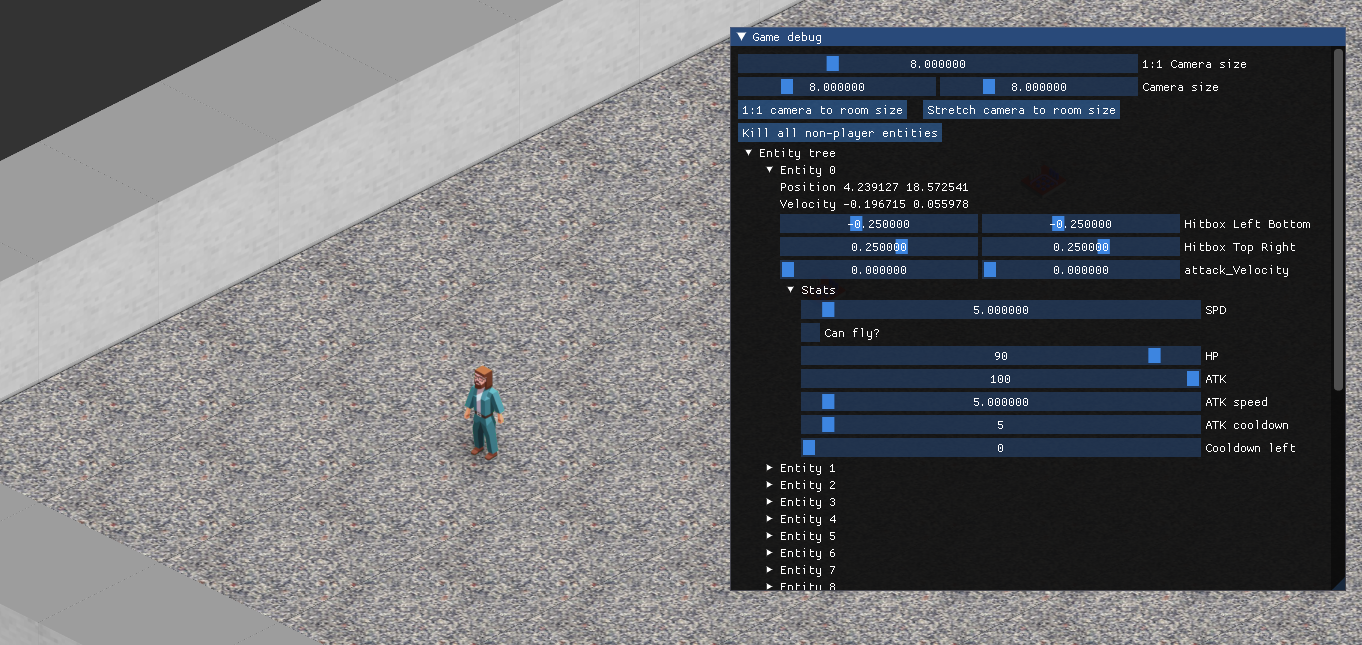
\includegraphics[scale=0.3]{images/debugwindow.png}
\centering
\caption{\textit{An instance of the debug window(character statistics showing)}}
\end{figure}
By implementing the testing as a two-step process, any feature added to the main pipeline is going to be tested both as a stand-alone piece of code, but also as part of an overarching program. By thoroughly checking most of the scenarios which can appear during gameplay, we know that the project version in the main extension branch is working, thus optimizing any future testing.
\subsection{Third-party code}
Although we wanted to get straight into coding, there was one huge challenge we were yet to face: \textbf{C would not be a programmer's first choice for game development}, due to the lack of OOP features. We decided on using necessary libraries such as \href{https://www.opengl.org}{\textbf{OpenGL}} for rendering, a C wrapper for the C++ library \href{https://www.dearimgui.com}{\textbf{Dear ImGui}}  (CImGui), \href{https://www.openal.org}{\textbf{OpenAL}} for the audio, and \href{https://www.glfw.org}{\textbf{GLFW}} for system input and window handling.

\section{Group reflection}
\subsection{Communication and task distribution}
Similarly to the emulator, we mostly communicated through face-to-face meetings in either labs or student accommodation, as well as a Whats App group chat, through which we could send updates or plan future meetings.\par
The initial task distribution was mostly done considering our previous experience with coding, Michał taking on the task of \textbf{rendering}, Jakub starting on the \textbf{collision detection}, Bogdan implementing the \textbf{pathfinding}, while Vlad started on the \textbf{room generation}. After somebody finished their tasks, they would check the backlog of features that needed implementation, and confer with the team in choosing the most necessary one in the current state of the project.
\subsection{Future improvements}
Having decided on an ambitious extension, we didn't know how much time it would take to produce the final version. As a consequence, \textbf{we rushed to finish every feature as swiftly as we could}, a strategy which worked well in the first couple of days, but we quickly realized that this was leading to burnout, so we started portioning the work much more. If we were to restart this project having all the previous knowledge, we would definitely work with a steady pace, albeit slower, rather than rush to finish features and spend more time recovering. \par
Another issue we faced was regarding \textbf{working in parallel on co-dependent features} (\textit{ex. the rendering and the entities}), which more often than not led to miscommunication, and convincing one another to change their implementation. We didn't find a general solution to this problem, especially towards the final submission date, as everything depended on previously implemented features, however, during the middle stages of development, we tried to assign new features to the person having already implemented their "dependency", so there would be fewer conflicts.

\section{Individual reflection}
\subsection{Bogdan Gavra}
Given that the entire group was acquainted before the project started, the need to get to know each other was already fulfilled. This meant that we were able to start working with a high level of compatibility from the very start, deciding on task distribution being done with everybody's agreement.\par
Personally, I believe that I fit into the group quite well and that I managed to successfully fulfill the roles assigned to me (implementing efficient pathfinding, finding appropriate textures, as well as adding character dialogue), and writing code that could be understood by the rest of the team. Also, I was pleasantly surprised to see that the team had the same enthusiasm about this project, especially the extension, which made working with them so much more enjoyable.\par
However, the constant work to ensure a presentable extension resulted in a short period of burnout, which made me feel that I was letting the team down, but I appreciate the team for being very supportive of this, and thus I tried to compensate for this after my recovery.
\subsection{Michał Andryskowski}
I was excited when my group members agreed to develop a game as our extension. I had experience with the libraries we were going to use, especially OpenGL. I tried my best to ensure that my teammates could compile the required libraries on their machines. It took a couple of sleepless nights (for me and the others) to solve all the strange issues specific to our target platforms but I think this period of crunch was unavoidable and I am glad we had a solid foundation to build on later on. \par
Communication was excellent, we would always question each other whenever a new feature was added and it felt like a professional environment. We rarely got stuck on solving a single bug as the code base was clear to all of us. \par
I see only one solution to solving our burnout without sacrificing the quality of the project - we would need to gain more experience working as a team so that we can trust each other more. For me the biggest contributor was worrying about miscommunication, which might have helped to avoid it happening, but at a price.
\subsection{Jakub Łapiński}
I think I fit into our group reasonably well. My communication with team members was smooth, as we knew each other before the project started. I could fill the group’s needs well, as my parts of the project were assigned flexibly according to the most urgent. I was thrilled when we decided that our extension should be a game. \par
Initially, was a bit overwhelmed by the task at the beginning, but our team overcame the difficulties thanks to great teamwork and communication. Our vision of the game was coherent and I fitted well into implementing the game’s physics. Unfortunately in the later parts of the extension, the initial urge to finish as much of the game as possible led to a burnout. As a solution to this problem I would set the time for work and free time to ensure that nobody is exhausted by, huge amounts of work.
\subsection{Vlad Marchis}
This project was quite challenging in terms of the progression rate. I did not expect to be part of such an amazing and driven team. Knowing each other beforehand played a large role as it eliminated any sort of uncomfortable situations. Consequently, we were straightforward with our questions or requests which made for an efficient and pleasurable work environment.  \par
I found the contents of the first half to be comprehensive and helped build a consistent foundation. Furthermore, I am glad about learning more about \href{https://gitlab.doc.ic.ac.uk/}{\textbf{GitLab}} and how to use it professionally. The Raspberry Pi task proved more complex than expected as we had mistakenly reformatted the provided SD Card and took a while (7 days) to notice. Moreover, we were among the first teams to start this task and therefore used the inaccurate information initially provided by the spec.\par
Overall, I thoroughly enjoyed the time spent on the project and the freedom of choosing our own extension and made up for a great end of the first year.

\end{document}
